\chapter{Sistemas operativos en tiempo real y FreeRTOS}


\section{FreeRTOS}
\subsection{Introducción}

\subsubsection{Qué es un sistema operativo en tiempo real}

Para poder entender con mayor completitud lo que significa un sistema operativo en tiempo real, es importante tener claro qué son en principio los sistemas operativos en sí. Y luego entrar a especificar detalles o conceptos como tiempo real y demás.

\subsubsection{Sistema operativo}

Un sistema operativo es un programa de computadora que soporta las funciones básicas de un computador, y proporciona servicios básicos a otros programas o aplicaciones que son los que se ejecutan en la computadora. Las aplicaciones son las que proporcionan las funcionalidades que el usuario requiere o necesita. Los servicios proporcionados por el sistema operativo hacen que escribir las aplicaciones sea más rápido, más simple y más fácil de mantener.\\

Una aplicación como por ejemplo navegador web, provee las funcionalidades para leer correos, visitar páginas, etc. Este navegador en sí mismo está siendo ejecutado dentro de un entorno que es el que el sistema operativo proporciona.

\subsubsection{Qué es un RTOS}

La mayoría de sistemas operativos permiten la ejecución de varios programas al mismo tiempo. La llamada multi tarea (multitasking). En realidad, cada núcleo del procesador puede estar ejecutando un solo hilo de procesamiento al tiempo. Un elemento del sistema operativo llamado planificador (scheduler) es el responsable de decidir cuál programa se ejecuta y cuándo se ejecuta, y proporciona la sensación de de ejecución simultánea mediante cambios en los programas.\\

El tipo de sistema operativo se define por cómo hace el planificador para decidir cuál programa se ejecuta y cuándo se ejecuta. \\

El planificador de un sistema operativo en tiempo real está diseñado para proveer un patrón de ejecución predecible o normalmente descrito como determinista. Esto es de particular interés en para los sistemas embebidos ya que estos generalmente tienen requerimientos de tiempo real. Un requerimiento de tiempo real es aquel que especifica que un sistema embebido debe responder a cierto evento dentro de un tiempo estrictamente definido (este se conoce como 'deadline'). La garantía total del cumplimiento del requerimiento de tiempo real solamente se puede dar si el comportamiento del planificador del sistema operativo puede ser predicho (en otras palabras que sea determinista).

Los planificadores tradicionales de los sistemas operativos en tiempo real (como el del sistema operativo FreeRTOS, cumple con el requisito de determinismo gracias a que permite al usuario asignar cierta prioridad a cada hilo de ejecución. El planificador hace uso de estas prioridades para conocer cuál es el siguiente hilo que se va a ejecutar. En FreeRTOS un hilo de ejecución se llama tarea o 'task'.\\

\subsubsection{Qué es FreeRTOS}

Es un tipo de sistema operativo en tiempo real diseñado para ser lo suficientemente pequeño para poder ser ejecutado en un microcontrolador. Aunque no está estrictamente limitado a uso exclusivo en MCU. \\

Un MCU es pequeño y restringido en recursos; típicamente el programa es ejecutado desde la ROM. Los MCU son utilizados en sistemas profundamente embebidos, estas son aplicaciones en las que realmente no se ve el procesador como tal o el software que se está ejecutando. Normalmente tienen un trabajo especifico, especializado y dedicado para hacer. Las restricciones de tamaño y naturaleza dedicada de aplicación raramente justifican el uso de una implementación completa de FreeRTOS. De hecho hace que sea posible la implementación total de un RTOS. El sistema FreeRTOS proporciona por tanto la funcionalidad de planificación en tiempo real del núcleo, intercomunicación de tareas, temporización y sincronización. 



\subsection{Fundamentos de RTOS}

En esta sección se realiza una breve introducción a los conceptos de multi tarea en tiempo real.

\subsubsection{Multitasking}

El \textbf{kernel} es el componente central dentro de un sistema operativo. Los sistemas operativos como Linux emplean kernels que permiten a los usuarios acceder al computador de manera aparentemente simultáneamente. Múltiples usuarios pueden ejecutar varios programas aparentemente concurrentemente. \\

Cada programa en ejecución es una tarea o \textbf{task} bajo el control del sistema operativo. Si un OS puede ejecutar múltiples tareas de esta forma, se denomina \textbf{multitasking}.\\

El uso de un SO multitasking puede simplificar el diseño de lo que podría ser una aplicación bastante más complicada de otra manera:

\begin{itemize}
    \item El multitasking y la comunicacion entre tasks permiten a una aplicación compleja ser separada en un conjunto de tareas más pequeñas y más manejables.
    \item La partición de tareas puede resultar en pruebas de software más sencillas de realizar, y en reutilización de código.
    \item Se pueden eliminar detalles complejos de temporización y secuenciación del código de la aplicación y convertirse en una responsabilidad del sistema operativo.
\end{itemize}

\paragraph{Multitasking vs concurrencia}

Un procesador convencional puede ejecutar solamente una tarea al tiempo, pero intercambiando rápidamente entre tareas, un sistema multitasking puede dar la apariencia de estar ejecutando varias tareas de manera concurrida. Esto se representa en el diagrama siguiente. Este diagrama muestra el patrón de ejecución de tres tareas con respecto al tiempo. 

\begin{figure}[H]
    \centering
    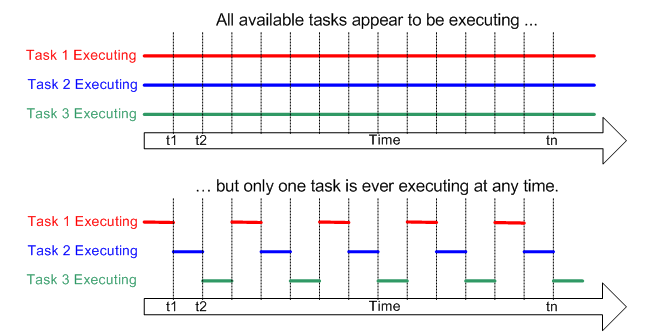
\includegraphics[scale=0.7]{RTOS/f1.PNG}
\end{figure}

\subsubsection{Planificación}

El planificador es la parte del kernel responsable de decidir cuál es la tarea que se ejecuta en cualquier tiempo específico. El kernel puede suspender y más adelante reanudar cualquier tarea muchas veces durante el tiempo de vida de la tarea.\\

La política de planificación es el algoritmo utilizado por el planificador para tomar la decisión de cuál es la tarea que se ejecutará en cualquier punto del tiempo. La política de planificación de un sistema multi usuario en tiempo no real lo más probable es que permita a cada tarea una proporción "justa" del tiempo de provesamiento. \\

Adicionalmente a ser suspendido por el kernel de manera involuntaria, una tarea puede escoger suspenderse a sí misma. Esto lo hará si necesita retardar (\textbf{sleep}) un periodo fijado de tiempo o esperar (\textbf{block}) para que algún recurso se vuelva disponible (por ejemplo un puerto serial) o que algún evento ocurra (por ejemplo una señal proveniente). Una tarea bloqueada o dormida no puede ejecutarse y no tomara parte de tiempo de procesamiento.  

\begin{figure}[H]
    \centering
    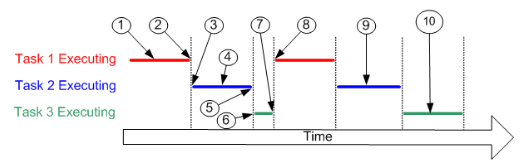
\includegraphics[scale=1]{RTOS/f2.PNG}
\end{figure}

los tiempos marcado en la imagen anterior son:

\begin{itemize}
    \item En (1) se ejecuta la tarea 1.
    \item En (2) el kernel suspende (intercambia) la tarea 1.
    \item Y el el mismo tiempo continúa la tarea 2.
    \item Mientra se ejecuta la tarea 2 en el tiempo (4) bloquea los periféricos del procesador para su acceso exclusivo.
    \item en (5) y (6) se suspende tarea 2 y reanuda tarea 3.
    \item La tarea 3 trata de usar recursos de periféricos, al ver que no está disponible, se suspende en el tiempo (7).
    \item En el tiempo (8) se reanuda tarea 1.
    \item En el tiempo (9) la tarea 2 finaliza el uso del periférico y entonces lo desbloquea.
    \item En (10) la tarea 3 ya encuentra disponibilidad de periféricos y puede ejecutarse.
\end{itemize}

\subsubsection{Cambio de contexto}

Al ejecutarse una tarea esta utiliza recursos del procesador o microcontrolador tales como registros y accede a la memoria RAM y ROM de igual manera que cualquier otro programa. Estos recursos comprenden el \textbf{contexto} de la ejecución de la tarea.

Una tarea es una porción de código secuencial, este no sabe cuándo será suspendido (o intercambiado por otra tarea) o reanudado por el kernel; incluso no sabe si estas suspensiones o reanudaciones ocurrieron. Considerando un ejemplo en que una tarea es suspendida por el kernel justamente antes de ejecutar una instrucción que realiza la suma de los valores de dos registros del procesador. Mientras la tarea está suspendida otras son ejecutadas y pueden modificar los valores contenidos en estos registros. Tras la reanudación de la tarea, esta no sabrá que los valores de los registros fueron cambiados. Es importante tener esto en cuenta porque si la tarea asume que los valores no se cambiaron, el valor de la suma no será correcto. \\

Para prevenir este tipo de posibles errores es esencial que al reanudarse una tarea tenga un contexto idéntico al que tenía antes de ser suspendido. El kernel del sistema operativo es el responsable de asegurar estas condiciones y lo realiza guardando el contexto de la tarea antes de suspenderla. Una vez se reanuda, este contexto se restaura por el sistema operativo. Este proceso de guardar y cargar el contexto de cada tarea se llama intercambio de contexto.

\subsubsection{Aplicaciones de Tiempo Real}

Los Sistemas Operativos en Tiempo Real logran ser multi-tarea a través de los anteriores principios, pero sus objetivos son muy diferentes a aquellos que no son tiempo real. El objetivo diferente se refleja en la política de planificación. Los sistemas embebidos y de tiempo real están diseñados para proporcionar una respuesta oportuna a eventos del mundo real. Estos eventos del mundo real pueden tener tiempos de terminación antes de los cuales el sistema embebido debe responder y la política de planificación RTOS tiene que asegurar que estos plazos o tiempos de terminación se cumplan. \\

Para lograr lo anterior el diseñador(a) de software le debe asignar un nivel de prioridad a cada tarea. La política de planificación del RTOS se asegura entonces de que la tarea con más alta prioridad se pueda ejecutar en el tiempo de procesamiento de la tarea dado. Esto puede requerir que se comparta tiempo de procesamiento "equitativo" entre tareas que tengan misma prioridad si ambas están listas para ejecutarse.

\paragraph{Ejemplo} El ejemplo más básico de RTOS es un sistema que incorpora un teclado y un LCD. Un usuario debe tener retroalimentación visual de cada tecla presionada dentro de un periodo de tiempo razonable. Si el usuario no puede ver que la tecla presionada ha sido aceptada dentro de este tiempo, el software será, en el mejor de los casos, incómodo de usar. Si el tiempo máximo aceptable era de 100ms, cualquier respuesta que esté por debajo de este tiempo será considerado como aceptable. Esta funcionalidad puede ser implementada como una tarea autónoma con la siguiente estructura.

\begin{verbatim}
    void vKeyHandlerTask( void *pvParameters )
    {
    // Key handling is a continous process and as such the task \\
    // is implemented using an infinite loop (as
    // most real time tasks are) \\
    for( ;; )
    {
        [suspend waiting for a press key]
        [process the key press]
    }
    }
\end{verbatim}

Ahora asúmase que el sistema en tiempo real también está llevando a cabo una unción de control que se basa en una entrada digital filtrada. Esta entrada debe ser muestreada, filtrada, y el ciclo de control ejecutado cada 2ms. Para una correcta operación de filtro, la regularidad temporal de la muestra debe ser precisada a 2.5ms. Esta funcionalidad debe ser implementada como una tarea autónoma con una estructura similar a la anterior: \\

\begin{verbatim}
    void vControlTask( void *pvParameters )
    {
        for( ;; )
    {
        [suspend waiting for 2ms since the start of the previous cycle]
        [sample the input]
        [filter the signal]
        [perform control algorithm]
        [output result]
    }
    }
\end{verbatim}

El diseñador de software debe asignar a la tarea de control una prioridad mayor ya que:

\begin{enumerate}
    \item El plazo de tiempo para la tarea de control es más estricta que la de la lectura de tecla.
    \item La consecuencia de no cumplir el plazo de tiempo es mayor para la tarea de control que para la otra.
\end{enumerate}

\subsubsection{Planificación de tareas}

\begin{figure}[H]
    \centering
    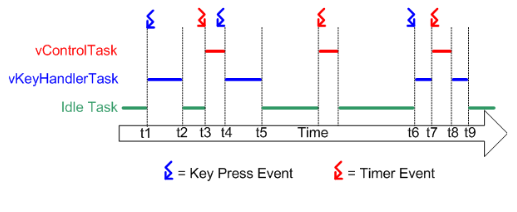
\includegraphics[scale=1]{RTOS/f3.PNG}
\end{figure}

El diagrama muestra cómo deberían ser planificadas las tareas por el sistema de tiempo real. El RTOS crea por sí mismo una tarea llamada \textbf{idle} task (tarea de inactividad) la cual se ejecuta solamente cuando no hay ninguna otra tarea ejecutándose o disponibles. Esta tarea siempre está en un estado en el que puede ejecutarse. \\

\begin{itemize}
    \item Al inicio ninguna de las dos tareas se está ejecutando ni están disponibles para ejecución, por ello la tarea actual es \textbf{idle}. Pues vControlTask está esperando para el momento correcto de arranque de un nuevo ciclo de lectura y vKeyHandlerTask está esperando a que se oprima una tecla.
    \item En t1 se presiona una tecla. vKeyHandlerTask ahora está disponible para ejecutarse, tiene una prioridad mayor que \textbf{idle} task. 
    \item en t2 vKeyHandlerTask completa su proceso de tecla y visualización en LCD. No puede continuar hasta que sea presionada otra tecla, así que se auto suspende y se reanuda la tarea inactiva. 
    \item En t3 un evento de temporización indica que es tiempo de ejecutarse el siguiente ciclo de control. vControlTask ahora está disponible y como tiene la mayor prioridad entonces el planificador da el tiempo de ejecución de procesamiento.
    \item Entre t3 y t4, mientras vControlTask se está ejecutando, se presiona una tecla. Eso significa que vKeyHandlerTask pasa a estar disponible para ejecución, pero como tiene un nivel de prioridad menor, entonces no se le asigna un tiempo de procesamiento por el planificador.
    \item En t4 el proceso de control termina su ejecución y no puede reiniciar hasta el siguiente evento de temporización; por tanto se suspende a sí mismo. vKeyHandlerTask ahora es la tarea con la mayor prioridad disponible para ejecutarse, por ende el planificador le da tiempo de procesamiento e inicia su ejecución. 
    \item En t5 se termina el proceso de la tecla y vKeyHandlerTask se suspende para esperar siguiente evento. No hay tareas así que se ejecuta 'inactiva'
    \item En el tiempo t6 se presiona otra tecla, pero en medio del procesamiento de la tarea, el evento de temporización de control se dispara, entonces por sus prioridades indican, el planificador le da tiempo de procesamiento a vControlTask y suspende vKeyHandlerTask guardando su contexto para poder seguir siendo ejecutado después.
\end{itemize}

\subsection{Implementación de RTOS}

Esta sección describe el código fuente de intercambio de contextos de un RTOS desde el inicio. En este ejemplo se utiliza el MCU Atmel AVR con el puerto de FreeRTOS. La sección finaliza con un vistazo muy detallado paso por paso de un cambio de contextos completo.

\subsubsection{Tipos de datos}

Cada puerto FreeRTOS tiene un único archivo cabecera \texttt{portmacro.h} el cual contiene (entre varias otras cosas) definiciones de dos tipos de variables específicos: \texttt{TickType\_t} y \texttt{BaseType\_t}.

\paragraph{\texttt{TickType\_t}}

El sistema operativo siempre configura una interrupción periódica, se conoce con el nombre de interrupción de tick. El número de interrupciones de tick que han ocurrido desde que el sistema RTOS inicia se llama contador de tick. Este contador se utiliza como una medida de tiempo. El tiempo entre una interrupción de tick y la siguiente se denomina periodo de tick. Y los tiempos se especifican como múltiples periodos de tick.\\

\texttt{TickType\_t} es el tipo de dato utilizado para contener el valor de conteo de ticks y para especificar tiempos. Este tipo de dato puede ser de 16 bits sin signo o de 32 bits sin signo, dependiendo del parámetro de configuración de \texttt{configUSE\_16\_BIT\_TICKS} en \texttt{FreeRTOSConfig.h}; si su valor es 1, entonces \texttt{TickType\_t} es un \texttt{uint16\_t}, si el valor es 0 entonces será \texttt{uint32\_t}.

\paragraph{\texttt{BaseType\_t}}

Este siempre se define como el tipo de dato más eficiente para la arquitectura. Típicamente es un dato de 32 bits, y si la arquitectura es menor, entonces será de este tamaño. \texttt{BaseType\_t} se usa generalmente para retornar tipos de datos que solamente puede tomar un rango muy limitado de valores, y valores booleanos \texttt{pdTRUE/pdFALSE}.\\

Algunos compiladores.

\paragraph{Nombres de funciones}

Lasfunciones tienen diferenes prefijos y cada uno indica el tipo de dato de retorno, y el archivo sobre el que está definido. Por ejemplo

\begin{itemize}
    \item \texttt{vTaskPrioritySet()}: la 'v' indica que retorna un \texttt{void} y está definido dentro de \textbf{task.c}.
    \item \texttt{xQueueReceive()}: la 'x' indica que el retorno es del tipo \texttt{BaseType\_t} y está definido dentro de \textbf{queue.c}.
    \item \texttt{pvTimerGetTimerID()} la 'p' y la 'v' indican que el retorno es un puntero a un \texttt{void} y está definido dentro de \textbf{timers.c}
\end{itemize}

Funciones privadas en un entorno tienen el prefijo 'prv'.

\paragraph{Nombres de macro}

La mayoría de los macros están escritos en mayúsculas y tienen prefijos con letras minúsculas que indican dónde está definido dicho macro. 

\begin{itemize}
    \item \texttt{portMAX\_DELAY)} es un macro que está definido en \texttt{portable.h} o en \texttt{portmacro.h}.
    \item \texttt{taskENTER\_CRITICAL()} está definido en \texttt{task.h}.
    \item \texttt{pdTRUE} en \texttt{projdefs.h}.
    \item \texttt{configUSE\_PREEMPTION)} en \texttt{FreeRTOSConfig.h}
    \item \texttt{errQUEUE\_FULL)} en \texttt{projdefs.h}.
\end{itemize}

Note que las funciones API de los semáforos están escritas casi enteramente como un conjunto de macros, aunque siguen la convención de nombres de funciones. 

\subsubsection{Piezas de armado}

\paragraph{Herramientas de desarrollo}

Un objetivo de FreeRTOS es que sea simple y sencillo de entender. Para este fin la mayoría de códigos fuente de sistemas operativos en tiempo real están escritos en C. \\

El ejemplo presentado en esta sección utiliza una herramienta de desarrollo para windows de AVR.

\paragraph{El tick de RTOS}

Cuando está en modo inactivo (sleeping) una tarea de tiempo real va a especificar un tiempo después del cual requerirá 'despertar'. Cuando está bloqueado, la tarea puede especificar un tiempo máximo el cual desea esperar.\\

El kernel de FreeRTOS mide el tiempo en unidades básicas llamadas \textbf{ticks}. Una interrupción de tiempo (tick interrupt) incrementa el conteo de ticks con una estricta precisión del tiempo. Permitiendo al kernel medir el tiempo con una resolución de la frecuencia de la interrupción. \\

Cada vez que el contador de ticks incrementa el kernel del sistema operativo debe evaluar y ver si es momento de desbloquear o despertar una tarea. Es posible que una tarea despertada o desbloqueada durante el tick ISR tenga una prioridad más alta que aquella relacionada con la tarea interrumpida. Si este es el caso el tick ISR deberá retornar a la tarea recien despertada o desbloqueada, interrumpiendo efectivamente una tarea pero regresando a otra.


\begin{figure}[H]
    \centering
    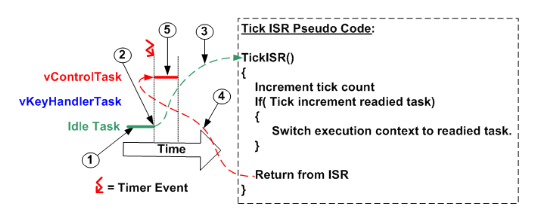
\includegraphics[scale=1]{RTOS/f4.PNG}
\end{figure}

\begin{itemize}
    \item En (1) se está ejecutanto la tarea inactiva de RTOS.
    \item En (2) ocurre un tick de RTOS (evento o interrupción) y el control transfiere al ISR (3).
    \item El ISR de la interrupción por temporización hace que vControlTask esté lista para ejecutarse, y como esta tarea tiene mayor prioridad que la inactiva, se hace el cambio de contexto al de vControlTask.
    \item Como el contexto de ejecución ahora es el de la tarea vControlTask, saliendo del ISR (4) retorna el control a vControlTask, el cual empieza a ejecutarse.
\end{itemize}

Un cambio de contexto de ejecución que ocurre de esta manera se denomina preventiva \textbf{preemptive} ya que la tarea interrumpida es cambiada pero sin suspenderse voluntariamente.

El puerto AVR de FreeRTOS utiliza un evento de comparación en un temporizador para generar el tick.

\paragraph{Atributos de señal GCC}

Las interrupciones pueden ser escritas en C gracias a la herramienta de desarrollo GCC. Un evento de coincidencia del periférico timer 1 del AVR puede ser escrito de la siguiente forma.

\begin{verbatim}
    void SIG_OUTPUT_COMPARE1A( void ) __attribute__ ( ( signal ) );
    
    void SIG_OUTPUT_COMPARE1A( void )
    {
        /* ISR C code for RTOS tick */
        vPortYieldFromTick();
    }
\end{verbatim}

Aquí, la directiva \texttt{\_\_attribute\_\_ ( ( signal ) )} lo que hace es \textbf{informar al compilador que la función es un ISR } y resulta en dos cambios importantes en la salida de compilación 

\begin{enumerate}
    \item El atributo de 'señal' asegura que cada registro del procesador que sea modificado durante la ejecución del ISR será restaurado a su valor original cuando la rutina de interrupcción termine. Esto es requerido ya que el compilador no puede hacer ninguna suposición sobre cuándo se va a ejecutar la interrupción, y por tanto no puede optimizar cuáles registros del procesador requieren salvado y cuáles no.
    \item El atributo 'señal' también fuerza una instrucción de "retorno después de interrupción" (RETI) para ser usada en lugar de la instrucción "return" (RET) que sería usada en otros casos. El controlador AVR deshabilita las interrupcciones al entrar en un ISR y la instrucción RETI es requerida para reactivarla al salir.
\end{enumerate}

\paragraph{GCC Naked Attribute}

En la sección anterior se muestra cómo el atributo de 'señal' puede ser usado para escribir un ISR en C y cómo esto resulta ser parte del contexto de ejecución siendo guardado o salvado (solamente los registros modificados por el ISR son salvados). Sin embargo, el intercambio de un contexto de ejecución requiere que el contexto completo sea salvado. \\

El código de la aplicación podría guardar explícitamente todos los registros del procesador del ISR entero, pero hacer esto podría resultar en registros del procesador guardándose dos veces, lo cual sería innecesario. Esto puede ser evitado utilizando el atributo \texttt{naked attribute}.

\begin{verbatim}
    
void SIG_OUTPUT_COMPARE1A( void ) __attribute__ ( ( signal, naked ) );

void SIG_OUTPUT_COMPARE1A( void )
{
    /* ISR C code for RTOS tick. */
    vPortYieldFromTick();
}
\end{verbatim}

Este atributo previene al compilador de generar código de entrada o salida de funciones. Cuando este atributo se usa, el compilador no genera ninguna línea de código de entrada o salida de funciones, así que toca hacerlo explícitamente. Los macros de RTOS \texttt{portSAVE\_CONTEXT()} y \texttt{portRESTORE\_CONTEXT()} guardan y recargan el contexto entero de ejecución.

\begin{verbatim}
    void SIG_OUTPUT_COMPARE1A( void ) __attribute__ ( ( signal, naked ) );

void SIG_OUTPUT_COMPARE1A( void )
{
    /* Macro that explicitly saves the execution
    context. */
    portSAVE_CONTEXT();

    /* ISR C code for RTOS tick. */
    vPortYieldFromTick();

    /* Macro that explicitly restores the
    execution context. */
    portRESTORE_CONTEXT();

    /* The return from interrupt call must also
    be explicitly added. */
    asm volatile ( "reti" );
}
\end{verbatim}


El atributo 'naked' le da al código de la aplicación un control completo sobre cómo y cuándo el contexto AVR se guarda. Si el código guarda el contexto entero al entrar a la ISR entonces no es necesario volerlo a guardar después de realizar un cambio de contexto, por lo que ningún registro del procesador se guarda dos veces. 

\paragraph{Código de tick de FreeRTOS}


El código fuente actual de FreeRTOS para el AVR es levemente diferente al mostrado en este ejemplo. \texttt{vPortYieldFromTick()} por sí mismo ya está implementada como una función "naked", y el contexto de ejecución se guarda y se recupera dentro de \texttt{vPortYieldFromTick()}. Está hecho de esta manera debido a la implementación de cambiadores de contexto no preventivos. 

\begin{verbatim}
/*--------------------------------------------------*/

/* Interrupt service routine for the RTOS tick. */
void SIG_OUTPUT_COMPARE1A( void )
{
    /* Call the tick function. */
    vPortYieldFromTick();

    /* Return from the interrupt.  If a context
    switch has occurred this will return to a 
    different task. */
    asm volatile ( "reti" );
}
/*--------------------------------------------------*/

void vPortYieldFromTick( void )
{
    /* This is a naked function so the context
    is saved. */
    portSAVE_CONTEXT();

    /* Increment the tick count and check to see
    if the new tick value has caused a delay
    period to expire.  This function call can
    cause a task to become ready to run. */
    vTaskIncrementTick();

    /* See if a context switch is required.  
    Switch to the context of a task made ready
    to run by vTaskIncrementTick() if it has a
    priority higher than the interrupted task. */
    vTaskSwitchContext();

    /* Restore the context.  If a context switch
    has occurred this will restore the context of
    the task being resumed. */
    portRESTORE_CONTEXT();

    /* Return from this naked function. */
    asm volatile ( "ret" );
}
/*--------------------------------------------------*/
\end{verbatim}

\paragraph{El contexto del AVR}

Un cambio de contexto requiere que todo el contexto de ejecución sea guardado. Para el ejemplo del MCU AVR el contexto consiste de

\begin{itemize}
    \item 32 registros de propósito general. La herramienta de desarrollo de GCC asume que el registro R1 está configurado a cero.
    \item Registro de estado. El valor de este registro afecta la ejecución de instrucción, y debe ser preservado a lo largo de lso cambios de contexto.
    \item Contador del programa. Al reanudarse una tarea, esta debe continuar la ejecución desde la instrucción que estaba a punto de ejecutarse inmediatamente previa a la suspensión. 
    \item Los dos apuntadores de la pila.
\end{itemize}

\subparagraph{Nota} \textit{call stack} o pila de llamadas es una estructura de datos de tipo pila (colección de elementos a los que se puede hacer push y pop) dinámica de tipo LIFO que almacena información sobre las subrutinas activas en un programa.

\begin{figure}[H]
    \centering
    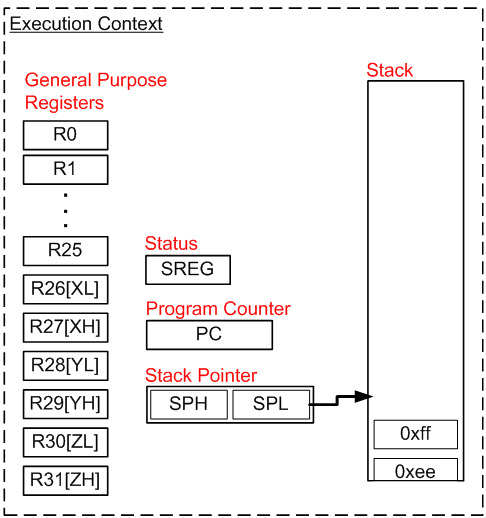
\includegraphics[scale=1]{RTOS/f5.PNG}
\end{figure}

\paragraph{Guardado del contexto}

Cada tarea de tiempo real tiene su propio espacio en la memoria de la pila así que el contexto puede guardarse simplemente haciendo "push" los registros del procesador en la pila de la tarea. \\

 \textit{portSAVE\_CONTEXT()} Está implementado como un macro para el AVR, cuyo código fuente es el siguiente
 
 \begin{verbatim}
#define portSAVE_CONTEXT()           
asm volatile (	                     
  "push  r0                    nt"  (1)
  "in    r0, __SREG__          nt"  (2)
  "cli                         nt"  (3)
  "push  r0                    nt"  (4)
  "push  r1                    nt"  (5)
  "clr   r1                    nt"  (6)
  "push  r2                    nt"  (7)
  "push  r3                    nt" 
  "push  r4                    nt" 
  "push  r5                    nt" 

    :
    :
    :

  "push  r30                   nt" 
  "push  r31                   nt" 
  "lds   r26, pxCurrentTCB     nt"  (8)
  "lds   r27, pxCurrentTCB + 1 nt"  (9)
  "in    r0, __SP_L__          nt"  (10)
  "st    x+, r0                nt"  (11)
  "in    r0, __SP_H__          nt"  (12)
  "st    x+, r0                nt"  (13)
);
 \end{verbatim}

Puntos importantes a considerar del código anterior:

\begin{itemize}
    \item El registro R0 se guarda primero
    \item El registro de estado es movido hacia R0 (2) para que pueda guardarse en la pila (4).
    \item Las interrupciones del procesador son deshabilitadas (3). Si \textit{portSAVE\_CONTEXT()} fue llamado solamente desde el contenido de una interrupción ISR, no habría necesidad de deshabilitar explícitamente las interrupciones. Mientras que si la macro se usa también por fuera de rutinas de interrupciones (cuando una tarea se suspende a sí misma) las interrupciones debes ser claramente deshabilitadas tan pronto como sea posible.
    \item El código generado por el compilador del código en C del ISR asume que el valor de R1 es cero. El valor original de R1 se guarda (5) antes de que se limpie (6).
    \item Entre (7) y (8) los reistros restantes se guardan en orden numérico.
    \item La pila de la tarea que se suspende ahora contiene una copia del contexto de ejecución de tarea. El kernel almacena el apuntador de la pila de la tarea, así el contexto puede ser recuperado cuando la tarea se reanude. El registo X se carga con la dirección hacia la cual el puntero se va a guardar. 
    \item El apuntador se guarda.
\end{itemize}

\paragraph{Restauración del contexto}

La macro \texttt{portRESTORE\_CONTEXT()} hace exactamente lo contrario a la anterior, restaura el contexto de una tarea una vez esté lista. Los registros que están almacenados en la pila de la tarea son recuperados por el kernel del SO y se almacenan de nuevo en los registros principales.

\begin{verbatim}
#define portRESTORE_CONTEXT()        
asm volatile (	
  "lds  r26, pxCurrentTCB      nt"  (1)
  "lds  r27, pxCurrentTCB + 1  nt"  (2)
  "ld   r28, x+                nt"  
  "out  __SP_L__, r28          nt"  (3)
  "ld   r29, x+                nt"  
  "out  __SP_H__, r29          nt"  (4)
  "pop  r31                    nt" 
  "pop  r30                    nt" 

    :
    :
    :

  "pop  r1                     nt" 
  "pop  r0                     nt"  (5)
  "out  __SREG__, r0           nt"  (6)
  "pop  r0                     nt"  (7)
);

\end{verbatim}

\begin{itemize}
    \item La variable \texttt{pxCurrentTCB} propia de FreeRTOS mantiene la dirección hacia donde el puntero de pila de la tarea puede recuperar. Este se carga en el registro X (1 y 2)
    \item El puntero de pila para la tarea que se va a resumir se carga al puntero de pila del AVR, primero el byte menos significativo y luego el más significativo.
    \item Los registros principales se establecen de la pila en orden inverso. 
    \item El registro de estado guardado en la pila entre lo registros R1 y R0 también se restauran.
\end{itemize}

\subsubsection{Ejemplo detallado}

En el siguiente ejemplo se muestra y se explica el cambio de un contexto de ejecución de tarea; de una tarea A de menor prioridad a una tarea B de mayor prioridad.

\paragraph{Antes de la interrupción por el tick}

Este ejemplo empieza con la tarea A ejecutándose. La tarea B había sido suspendida anteriormente por lo que su contexto ya se había guardado en su correspondiente pila.


\begin{figure}[H]
    \centering
    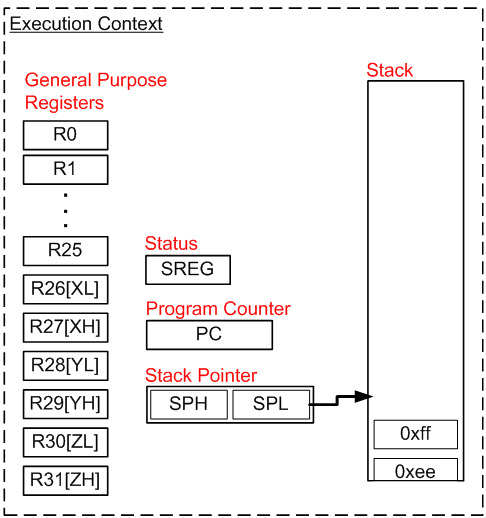
\includegraphics[scale=0.7]{RTOS/f5.png}
\end{figure}

Todo lo anterior corresponde a registros y datos que pertenecen al contexto de la tarea A.

\paragraph{La interrupción por tick ocurre}

el evento del tick de RTOS ocurre justo cuando la tarea A está a punto de ejecutar una istrucción LDI. Cuando la interrupción ocurre el MCU AVR sitúa automáticamente el contador del programa (PC) en la pila antes de dirigirse a la rutina de interrupción del tick.

\begin{figure}[H]
    \centering
    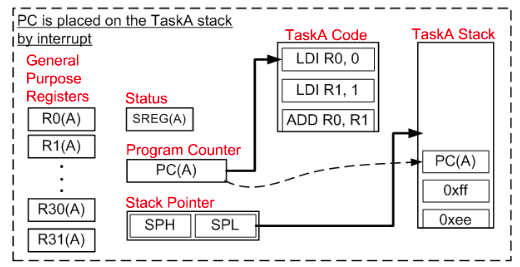
\includegraphics[scale=0.7]{RTOS/f6.PNG}
\end{figure}

\paragraph{Se ejecuta la interrupción del tick}

El código de la interrupción se puede ver a continuación.

\begin{verbatim}
/* Interrupt service routine for the RTOS tick. */
void SIG_OUTPUT_COMPARE1A( void )
{
    vPortYieldFromTick();
    asm volatile ( "reti" );
}
/*--------------------------------------------------*/

void vPortYieldFromTick( void )
{
    portSAVE_CONTEXT();

    vTaskIncrementTick();
    vTaskSwitchContext();
    portRESTORE_CONTEXT();

    asm volatile ( "ret" );
}
/*--------------------------------------------------*/
\end{verbatim}

la función \texttt{SIG\_OUTPUT\_COMPARE1A()} es del tipo 'naked', así la primera instrucción es un llamado al método \texttt{vPortYieldFromTick()} la cual es también 'naked' y el contexto de ejecución del AVR se guarda explícitamente a través del llamado a \texttt{portSAVE\_CONTEXT()}.

La función anterior guarda enteramente el contexto de ejecución en la pila de la tarea A. El puntero de esta pila apunta ahora al inicio de su propio contexto. \texttt{portSAVE\_CONTEXT} termina con guardar una copia del puntero de pila. El kernel de tiempo real ya tiene también una copia del puntero de pila de la tarea B que fue tomada en el momento en que esta fue suspendida.

\begin{figure}[H]
    \centering
    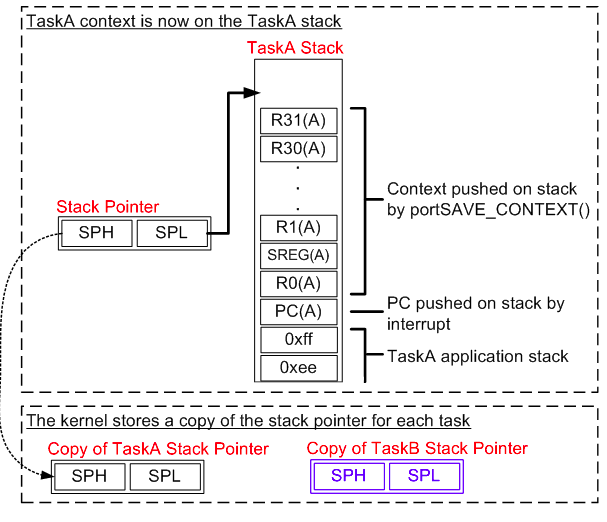
\includegraphics[scale=0.7]{RTOS/f7.PNG}
\end{figure}

\paragraph{Incremento del contador de Tick}

\texttt{vTaskIncrementTick()} se ejecuta después de que el contexto de la tarea A se guarda. Para los propósitos de este ejemplo se asume que el incremento del contador del tick ha causado que la tarea B se vuelva disponible para ser ejecutada. La tarea B tiene una prioridad mayor a la de A así que \texttt{vTaskSwitchContext()} selecciona a la tarea B para darle tiempo de ejecución al momento de que se complete la ISR.

\paragraph{Se recupera el puntero de pila de la tarea B}

\begin{figure}[H]
    \centering
    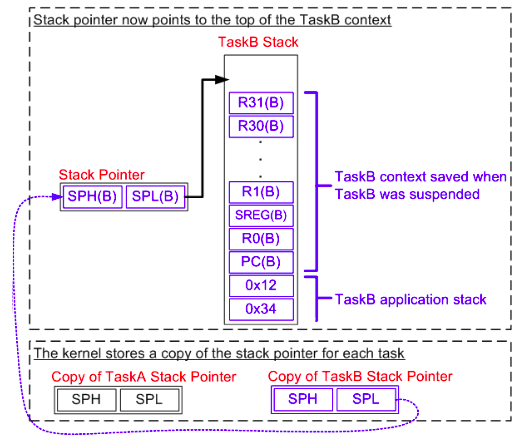
\includegraphics[scale=0.7]{RTOS/f8.PNG}
\end{figure}

Ahora la tarea B debe ser restaurada. Lo primero que hace la macro de RTOS \texttt{portRESTORE\_CONTEXT} es recuperar el puntero de pila de la tarea B de la copia que se había creado previamente a la suspensión de la tarea. El puntero de pila se carga al puntero de pila del procesador, ahora este apunta al tope del contexto de ejecución de Tarea B.

\paragraph{Restauración del contexto de B}

\texttt{portRESTORE\_CONTEXT()} se completa con la restauración del contexto de ejecución de la tarea B desde su pila hacia los registros principales correspondientes.

\begin{figure}[H]
    \centering
    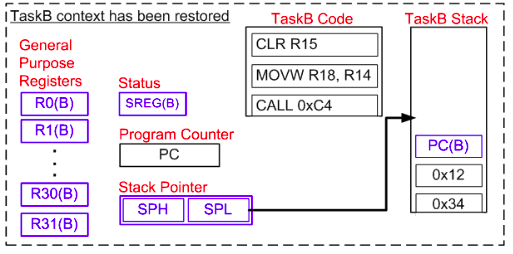
\includegraphics[scale=0.7]{RTOS/f9.PNG}
\end{figure}

Solamente el contador del programa es el que permanece en la pila de TaskB.

\paragraph{El tick de RTOS termina}

\texttt{vPortYieldFromTick()} retorna hacia \texttt{SIG\_OUTPUT\_COMPARE1A()} en la que la última instrucción es un retorno de interrupción \texttt{RETI}. Una instrucción de retorno de este tipo asume que el siguiente valor de la pila es una dirección de retorno que se puso en la pila cuando ocurrió la interrupción.

\begin{figure}[H]
    \centering
    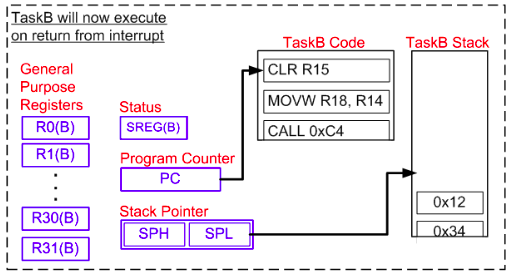
\includegraphics[scale=0.7]{RTOS/f10.PNG}
\end{figure}

Cuando la interrupción por tick empezó, el AVR automáticamente situó la dirección de retorno de la tarea A en la pila (la dirección de la siguiente instrucción a ejecutar de la tarea A). El manejador de tick de RTOS alteró el puntero de pila para que apuntara ahora a la pila de la tarea B. Entonces la dirección de retorno extraída de la pila por la instrucción RETI es ahora la dirección de instrucción de la tarea B que se iba a ejecutar inmediatamente antes de que fuera suspendida.  

\subsection{Concepto de las Tareas y co rutinas}

    \subsubsection{Introducción}
    
    Cada tarea es un pequeño programa. Tiene un puntero de entrada el cual se ejecuta en un blucle infinito normalmente. Una sola definición de una función \texttt{vTask} puede ser utilizada para crear cualquier número de tareas (cada tarea siendo una instancia separada de ejecución). \\
    
    Una aplicación puede tener varias tareas. Si el procesador que ejecuta la aplicación contiene solo un núcleo, entonces solamente se puede ejecutar una tarea al tiempo. 
    
    \paragraph{Características de una tarea}
    
    
    Una aplicación en tiempo real que utilice un RTOS puede estar estructurado como un conjunto de tareas independientes. Cada tarea se ejecuta dentro de su propio contexto sin ninguna dependencia de otras tareas en el sistema o en el planificador del sistema. Solamente una tarea dentro de la aplicación puede ser ejecutada en cualquier punto del tiempo y el planificado del sistema operativo de tiempo real es el responsable de decidir cuál es la tarea que se está ejecutando. El planificador por lo tanto puede iniciar y parar repetidamente cada tarea. Ya que una tarea no tiene conocimiento de la actividad del planificador, es la responsabilidad de este último asegurarse de que el contexto del procesamiento cuando una tarea vaya a ejecutarse sea el mismo contexto que había cuando la misma tarea dejó de ejecutarse en el pasado. Para cumplir con esto cada tarea tiene su propia pila.
    
    Cuando la pila es cambiada para dejar de ejecutar una tarea, el contexto de ejecución se guarda en esta pila.
    
    \paragraph{Características de una co-rutina}
    
    \subparagraph{Nota} Las co-rutinas fueron implementadas para el uso en dispositivos realmente pequeños, pero son usados muy raramente en la actualidad. \\
    
    Son conceptualmente muy similares a las tareas, y sus diferencias fundamentales son las siguientes
    
    \begin{enumerate}
        \item Uso de pila: Todas las corrutinas en una aplicación comparten una sola pila. Esto reduce grandemente el uso de memoria RAM del dispositivo.
        \item Planificación y prioridades: las rutinas de este tipo usan planificaciones cooperativas priorizadas con respecto a otras rutinas, pero pueden ser incluidas en aplicaciones que utilizan tareas. 
        \item La implementación de las corrutinas se proporciona a través de macros. 
    \end{enumerate}
    
    \subsubsection{Estados de una tarea}
    
    \paragraph{Ejecutando}
    
    Cuando una tarea se está ejecutando actualmente se dice que está en este estado. Está haciendo uso del procesador en ese momento. Si el procesador en el que se está ejecutando el RTOS tiene un solo núcleo entonces solo puede haber una tarea que esté en este estado.
    
    \paragraph{Lista}
    
    Las tareas en este estado son aquellas que tienen la posibilidad de ser ejecutadas, pero no se están ejecutando en ese momento porque otra tarea con una prioridad mayor es la que se está ejecutando. 
    
    \paragraph{Bloqueada}
    
    Se dice que una tarea está en este estado de bloqueo si en un tiempo está esperando por un evento sea externo o temporal. Por ejemplo si una tarea se llama \texttt{vTaskDelay()} esta estará bloqueada hasta que el periodo de delay haya expirado (evento temporal). Las tareas también se pueden bloquear para esperar una cola, semáforo, etc. Las tareas en este estado normalmente tienen un periodo de 'tiempo límite', después de este aunque el evento que sea que esté esperando no ocurra, esta tarea se desbloqueará.
    
    \paragraph{Suspendido}
    
    Así como las tareas que están en el estado de bloqueadas, aquellas que están suspendidas no pueden ser seleccionadas para entrar al estado de ejecución, la diferencia de este estado con el anterior es que no cuenta con un 'tiempo límite'. En lugar de eso las tareas solamente pueden entrar o salir de el estado suspendido cuando se les indica explícitamente en código, a través de \texttt{vTaskSuspend()} y \texttt{xTaskResume()}.
    
    
    \begin{figure}[H]
        \centering
        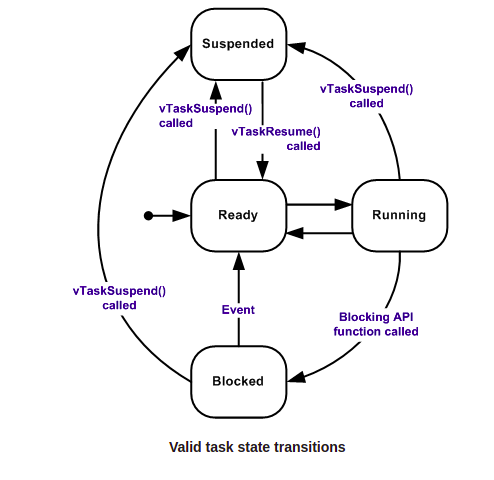
\includegraphics[scale=0.7]{RTOS/f11.PNG}
    \end{figure}
    
    
    \subsubsection{Prioridades de las tareas}
    
    A cada tarea se le asigna una prioridad que va desde 0 hasta \texttt{configMAX\_PRIORITIES} -1, donde \texttt{configMAX\_PRIORITIES} está configurado dentro de \texttt{FreeRTOSConfig.h}
    
    Si la tarjeta que se usa implementa un mecanismo de selección de tarea optimizada que utilice una instrucción del tipo "contador de ceros iniciales" y \texttt{configUSE\_PORT\_OPTIMISED\_TASK\_SELECTION} se establece en \texttt{1}, entonces \texttt{configMAX\_PRIORITIES} no puede ser mayor a 32. En todos los demás casos este puede tener cualquier valor.\\
    
    Números pequeños de prioridad denota tareas de baja prioridad. La tarea inactiva (idle task) tiene prioridad cero (\texttt{tskIDLE\_PRIORITY}). 
    
    El planificador del sistema operativo se asegura de que cualquier tarea que esté en estado Listo o Ejecutando siempre tenga su respectivo tiempo de procesamiento disponible en preferencia sobre las tareas que tengan una prioridad menor y que estén en el estado Lista. Dicho de otra forma, aquella tarea que esté en el estado Ejecución siempre será la tarea de mayor prioridad entre las que se encuentren listas o disponibles. 
    
    Pueden existir cualquier número de tareas que compartan la misma prioridad. Si el valor de \texttt{configUSE\_TIME\_SLICING } no está configurado o si su valor es igual a 1, entonces las tareas en el estado listas que tengan la misma prioridad compartirán el tiempo de procesamiento disponible mediante un esquema de planificación de turnos.
    
    \subsubsection{Planificación de las tareas}\label{plan_tar}
    
    El algoritmo de planificación es la rutina que decide cuál es la tarea que está en el estado ejecución. Solamente puede haber una tarea en este estado por cada núcleo de procesamiento. AMP (asymmetric multicore) es donde cada núcleo del procesador ejecuta su propia instancia de FreeRTOS. SMP (symmetric multicore) es donde hay una instancia de FreeRTOS que planifica las tareas a lo largo de los múltiples núcleos.
    
    \paragraph{Política por defecto de planificación para un núcleo}
    
    El sistema operativo utiliza una política de planificación de tareas con el mismo nivel de prioridad. Las palabras clave son "fixed-priority" "preemptive", "round-robin", "time-slicing".
    
    \begin{itemize}
        \item "Fixed priority" Significa que el planificador no cambia la prioridad de una tarea de forma permanente, aunque puede 'acelerar' temporalmente la prioridad de una tarea debido a herencia de prioridad.
        \item "Preemptive" Significa que el planificador siempre ejecuta la tarea de mayor prioridad que esté disponible o lista independientemente de cuándo puede volverse disponible. Por ejemplo si un ISR cambia la tarea disponible con más alta prioridad, el planificador va a detener la tarea actual de menor prioridad e inciará la de mayor.
        \item "Round-robin" significa que las tareas que tengan la misma prioridad se turnan para entrar en el estado de ejecución. 
        \item "Time sliced" significa que el planificador cambia de tareas de igual prioridad en cada interrupción de tick.
    \end{itemize}
    
    \subparagraph{Uso de planificador preventivo priorizado}
    
    Una de las consecuencias de que siempre se ejecute la tarea de mayor prioridad que esté disponible, es que una tarea de alta prioridad que nunca entra en los estados bloqueado o suspendido, va a estar permanentemente privando a las tareas de menor prioridad de tiempo de ejecución. Esta es una razón por la que normalmente siempre es mejor crear tareas que sean manejadas mediante eventos. Por ejemplo si una tarea de alta prioridad está esperando a que suceda un evento, no debería caer en un bucle por el evento gracias a que constantemente se está realizando sondeo, y tampoco en el estado de bloqueado o suspendido. En lugar de eso, la tarea debería entrar en el estado de bloqueado para esperar por ese evento. El evento puede ser enviado a la tarea a través de as primitivas de comunicación y sincronización inter tareas de FreeRTOS. Recibiendo el evento automáticamente se quita la tarea de alta prioridad del estado bloqueado. La tarea de prioridad más baja entonces se ejecutará mientras la de alta permanece en el estado bloqueado.
    
    \subparagraph{Configuración de la política de planificación RTOS}
    
    \begin{itemize}
        \item \texttt{configUSE\_PREEMPTION}: Si el valor de esta configuración se pone a cero entonces la configuración preventiva se apaga y el cambio de contextos solamente ocurrirá si la tarea en el estado ejecutando entra al estado de bloqueo o suspensión, la tarea en ejecución llama a la rutina \texttt{taskYIELD()}, o una ISR hace una solicitud manualmente para cambio de contexto.
        \item \texttt{configUSE\_TIME\_SLICING}: Si esta configuración se pone en cero, entonces los cortes (slicing) de tiempo se desactivan, de manera que el planificador no realizará cambios de tareas de igual prioridad en cada interrupción de tiempo.
    \end{itemize}
    
    \subsubsection{Implementación de una tarea}
    
    Una tarea deberá tener la siguiente estructura:
    
    \begin{verbatim}
        void vATaskFunction( void *pvParameters )
        {
            for( ;; )
            {
                -- Task application code here. --
            }
    
            /* Tasks must not attempt to return from their implementing
            function or otherwise exit.  In newer FreeRTOS port
            attempting to do so will result in an configASSERT() being
            called if it is defined.  If it is necessary for a task to
            exit then have the task call vTaskDelete( NULL ) to ensure
            its exit is clean. */
            vTaskDelete( NULL );
        }
    \end{verbatim}
    
    El tipo \texttt{TaskFunction\_t} se define como una función que retorna un void y toma un puntero void como su único parámetro. Todas las funciones que implementen una tarea deben ser de este tipo. El parámetro puede ser utilizado para pasar información de cualquier tipo hacia la tarea.
    
    Las funciones de tareas no deben tener un retorno, por lo que deberían ser siempre un bucle continuo. Sin embargo, como se indica en el apartado \ref{plan_tar}, normalmente es mejor crear tareas que sean manejadas por evento para no privar de tiempo de procesamiento a las tareas que tengan menor prioridad, a partir de la siguiente estructura:
    
    \begin{verbatim}
        void vATaskFunction( void *pvParameters )
        {
            for( ;; )
            {
                /* Psudeo code showing a task waiting for an event 
                with a block time. If the event occurs, process it.  
                If the timeout expires before the event occurs, then 
                the system may be in an error state, so handle the
                error.  Here the pseudo code "WaitForEvent()" could 
                replaced with xQueueReceive(), ulTaskNotifyTake(), 
                xEventGroupWaitBits(), or any of the other FreeRTOS 
                communication and synchronisation primitives. */
                if( WaitForEvent( EventObject, TimeOut ) == pdPASS )
                {
                    -- Handle event here. --
                }
                else
                {
                    -- Clear errors, or take actions here. --
                }
            }
    
            /* As per the first code listing above. */
            vTaskDelete( NULL );
        }
    \end{verbatim}
    
    Las tareas se crean mediante \texttt{xTaskCreate()} o \texttt{xTaskCreateStatic()} y se borran mediante \texttt{vTaskDelete()}.

\subsection{Colas y semáforos}

\subsubsection{Las colas en FreeRTOS}

Las colas son la forma principal y primaria de intercomunicación entre tareas. Pueden ser utilizadas para enviar mensajes entre tareas y entre tareas e interrupciones. En la mayoría de los casos son implementaciones de búferes FIFO. Cada nueva información a enviar se almacena al final del búfer, aunque también puede ser enviada al principio del mismo.\\

Las funciones de envío y recibimiento de datos a la cola: \texttt{xQueueSendToBack()} y \texttt{xQueueReceive()}

\paragraph{Modelo de usuario, simplicidad y flexibilidad}

El modelo de uso de las colas en FreeRTOS se administra para combinar simplicidad con flexibilidad. Los mensajes son enviados a través de las colas por copia, esto significa que los datos (los cuales pueden ser apuntadores a espacios grandes de memoria) son copiados en la cola, en lugar de la cola almacene solamente una referencia de los datos. Este es el mejor enfoque por las siguientes razones:

\begin{itemize}
    \item Mensajes pequeños que están ya de hecho contenidos en variables C (entero, estructura pequeña, etc) pueden ser directamente enviados a la cola. No hay necesidad de alojar esta información en un búfer para el mensaje y luego copiarla. De igual manera, los mensajes pueden ser leídos directamente desde la cola. Adicionalmente, esta forma permite por ejemplo soreescribir las variables que fueron enviadas a la cola, porque esa copia que se encuentra en la cola puede ser utilizada posteriormente.
    \item El uso de las colas que pasan la información mediante copia no quiere decir que no se pueda pasar información mediante referencia. Si por ejempli un mensaje es demasiadamente grande en tamaño como para ser copiado dentro de la cola, se puede definir en la cola para que esta maneje punteros hacia la información del mensaje y que estos punteros sean los que se envíen dentro de la cola.
    \item El kernel es completamente responsable de asignar la memoria utilizada como área de almacenamiento de las colas.
    \item Mensajes con tamaño variable pueden ser enviados configurando la cola de tal forma que permita tener estructuras que contengan un miembro que apunte al mensaje, y otro miembro que tenga el tamaño del mensaje.
    \item Una sola cola puede ser utilizada para recibir mensajes de distintos tipos, así como mensajes provenientes de distintas localizaciones, definiendo la cola para que contenga una estructura en la que un miembro es el tipo de mensaje y otro miembro que tenga el contenido del mensaje (o un puntero al mismo). La manera en la que se interpretan los datos depende del tipo de mensaje. 
    \item Esta implementación es naturalmente adecuada para el uso en un entorno de memoria protegida. Una tarea que está restringida a un área de memoria protegida puede pasar datos a una tarea que está restringida en otro área de memoria protegida porque invocar el RTOS llamando a la función de envío de cola aumentará el nivel de privilegio del MCU.Solo el sistema operativo (con todos los privilegios) accerde al área de almacenamiento de la cola.
    \item Un API separado o independiente está disponible para el uso dentro de las interrupciones.
\end{itemize}

\paragraph{Bloqueo en colas}

Las funciones API de colas permire que un tiempo de bloqueo sea especificado. Cuando una tarea trata de leer una cola que está vacía, la tarea entrará en el estado bloqueado (para que no consuma recursos de CPU y otras tareas puedan ser ejecutadas) hasta que alguna información o datos se haga disponible en la cola, o hasta que el tiempo de bloqueo expira.\\
Cuando una tarea trata de escribir en una cola que está llena, esta también entrará en el estado bloqueado hasta que haya espacio disponible en la cola o hasta que el tiempo de bloqueo expire.\\
Si más de una tarea se bloquea con la misma cola, entonces la tarea con mayor prioridad será la que se desbloquee primero. 

\subsubsection{Semáforos binarios}

Los semáforos binarios son utilizados tanto para exclusión mutua como para propósitos de sincronización. Los semáforos binarios y los mutex son muy similares excepto por unas pequeñas diferencias: los mutex incluyen un mecanismo de herencia prioritaria, mientras que los semáforos binarios no. Esto hace que los semáforos binarios sean el mejor recurso para implementar sincronización entre tareas o entre tarea e interrupción, y que los mutex sean la mejor opción para implementar exclusiones mutuas simples. \\

Las funciones de semáforo permiten que se especifique un tiempo de bloqueo. Dicho tiempo indica el número máximo de ticks (el tiempo) que una tarea deberá entrar en el estado de bloqueo cuando al tratar de 'tomar' un semáforo, este no esté inmediatamente disponible. Si más de una tarea se bloquea en el mismo semáforo, la tarea de mayor prioridad será la primera en ejecutarse cuando el semáforo esté disponible. \\

Se puede pensar en un semáforo binario como una cola que solamente puede tener un objeto almacenado. De esta forma la cola podrá estar solamente vacía o llena. A las tareas e interrupciones que usen la cola no les importará qué tiene la cola almacenada, solamente necesitan saber si esta está llena o vacía. \\

Considere el caso en que una tarea es usada para servir un periférico. Si se hace consulta repetitia (polling) al periférico esto gastaría innecesariamente recursos y evita que otras tareas puedan ser ejecutadas. Es preferible que la tarea permanezca más de su tiempo en el estado bloqueado (permitiendo a otras tareas ejecutarse) y solamente se ejecutará cuando verdaderamente haya algo que se deba hacer. Esto se logra mediante la implementación de un semáforo binario haciendo que la tarea se bloquee mientras trata de tomar el semáforo. Una rutina de interrupción es escrita para el periférico la cual activa el semáforo cuando el periférico necesita un servicio. la tarea siempre 'toma' el semáforo (el cual se puede interpretar como una lectura de la cola dejándola vacía), pero no puede escribirla. De este mismo modo la interrupción puede solamente escribir en la cola mas no leer de ella. \\

la prioridad de las tareas puede ser utilizada para asegurar que los periféricos sean servidos de manera oportuna.

\subsubsection{Semáforos contadores}

Así como los semáforos binarios pueden ser imaginados como una cola de un solo elemento, los semáforos contadores pueden ser imaginados como colas cuyo tamaño son mayores a uno. Nuevamente, los usuarios del semáforo no tienen interés de los datos que están almacenados en la cola, sino solo les interesa saber si está o no está vacía.\\

Los semáforos contadores son típicamente utilizados por las siguientes razones: \\

\begin{enumerate}
    \item Conteo de eventos: en este escenario de uso un manejador de tarea tomará un semáforo cada vez que procese un evento (decrementando el valor del semáforo). El valor del contador es la diferencia entre el número de eventos que han ocurrido, y el número que han sido procesados. En este caso es deseable que el valor del semáforo sea de cero cuando este es creado.
    \item administración de recursos: En este escenario el valor del contador indica el número de recursos disponible. Para obtener el control de un recurso, una tarea debe obtener primero un semáforo (decrementando el valor de su contador). Cuando el contador se hace cero, significa que ya no hay más recursos disponibles. Cuando la tarea termina de usar el recurso, se lo 'entrega' de nuevo al semáforo, aumentando nuevamente el valor del contador. En este caso es deseable que el valor del semáforo sea del máximo en el momento en el que es creado.
\end{enumerate}

\subsubsection{Mutex}

Los mutex son muy similares a los semáforos binarios que incluyen un mecanismo de herencia de prioridad. Mientras que los semáforos binarios son la mejor opción para implementar sincronización (entre tareas, o tarea-interrupción) los mutex son la mejor opción para implementar exclusiones mutuas sencillas. Cuando se usa para este propósito el mutex actúa como una 'ficha' para guardar un recurso. Cuando una tarea desea acceder al recurso primero debe obtener o 'tomar' la ficha. Cuando ha terminado de usar ese recurso, 'deja' o 'devuelve' la ficha de nuevo, con ello concede la oportunidad a otras tareas de obtener ese recurso.\\

Los mutex utilizan las mismas aplicaciones e API de los semáforos, así que también permite especificar un tiempo de bloqueo. Este tiempo indica el número máximo de ticks en que la tarea debería entrar al estado bloqueado cuando trata de 'pedir la ficha' del mutex si este no está disponible en ese momento. La herencia de prioridad significa que si una tarea de alta prioridad se bloquea mientras está esperando el mutex que está actualmente en manos de una tarea de menor prioridad, entonces la prioridad de la tarea es elevada temporalmente a aquella que está esperando la 'ficha'. Este mecanismo está diseñado para asegurar que la tarea de alta prioridad se mantenga en el estado bloqueado el menor tiempo posible.\\

\subsubsection{Mutex recursivos}

Un mutex utilizado de manera recursiva puede ser 'tomado' de manera repetida por el propietario. El mutex no se hace disponible de nuevo hasta que el propietario llama a la función \texttt{xSemaphoreGiveRecursive()} por cada solicitud de \texttt{xSemaphoreTakeRecursive()} satisfactoria. Por ejemplo, si una tarea 'toma' satisfactoriamente 5 veces entonces el mutex no estará disponible para ninguna otra tarea hasta que la tarea 'devuelva' ese mutex exactamente las 5 veces.\\

Este tipo de semáforo usa un mecanismo de herencia de prioridad, por lo que una tarea que 'toma' el semáforo \textbf{siempre tiene} que devolver el semáforo una vez no lo requiera más. Los semáforos tipo mutex no pueden ser utilzados desde el interior de una rutina de servicio de interrupción.\\

Los mutex no deberían ser usados en las interrupciones porque:

\begin{itemize}
    \item Incluyen un mecanismo de herencia de prioridad lo cual solamente tiene sentido si el mutex se toma o se recibe desde una tarea.
    \item Una interrupción no puede bloquearse para esperar un recurso.
\end{itemize}

\subsection{Notificaciones directas hacia tareas}

\subsubsection{Introducción}

Cada tarea de RTOS tiene un arreglo de notificaciones de tarea. Cada notificación de tarea tiene un estado que puede ser 'pendiente' o 'no pendiente' y un valor de notificación de 32 bits. la constante \texttt{configTASK\_NOTIFICATION\_ARRAY\_ENTRIES} configura el número de índices en el arreglo de notificaciones.\\

Una \textit{notificación directa a tarea} es un evento enviado directamente a la tarea, en lugar de enviarla indirectamente mediante un objeto intermediario como por ejemplo una cola, un grupo de eventos o un semáforo. Al enviar una notificación directa a una tarea el estado de la notificación de la tarea pasa a ser 'pendiente'. Así como una tarea se puede bloquear en un objeto intermediario como un semáforo para esperar a que el semáforo esté disponible, también puede bloquearse en una notificación de tarea para esperar a que el estado de dicha notificación se vuelva pendiente.\\

Con el envío de notificaciones directas hacia tareas, opcionalmente se puede actualizar el valor de la notificación objetivo de las siguientes maneras:

\begin{itemize}
    \item Sobreescribir el valor sin importar si la tarea ya ha leído el valor que se va a sobreescribir o no.
    \item Sobreescribir el alor, pero solamente si la tarea ya leyó el valor que se va a asobreescribir.
    \item Cambiar uno o mas bits en el valor.
    \item Incrementar el valor en 1.
\end{itemize}

Al llamar \texttt{xTaskNotifyWait()/xTaskNotifyWaitIndexed()} para leer el valor de una notificación, borra el estado de esa notificación a 'no pendiente'. El estado de la notificación también puede cambiarse a 'no pendiente' explícitamente mediante \texttt{xTaskNotifyStateClear()/xTaskNotifyStateClearIndexed()}.

Cada notificación dentro del arreglo opera de forma independiente - una tarea solo puede bloquearse en una notificación dentro del arreglo al tiempo y no podrá ser desbloqueada por una notificación enviada a otro índice del arreglo.\\

Estas notificaciones están por defecto habilitadas y se pueden excluir del programa configurando \texttt{ configUSE\_TASK\_NOTIFICATIONS } a cero.

\subsubsection{Restricciones y beneficios}

La flexibilidad de las notificaciones permiten que puedan ser usadas cuando, de lo contrario, habría sido necesario crear una cola separada, un semáforo binario, de conteo o un grupo de eventos. El uso de las notificaciones directas es más rápido (45\%) más rápido. Por supuesto también existen agunas limitaciones:

\begin{enumerate}
    \item Las notificaciones solamente pueden ser utilizadas cuando solamente hay una tarea que puede ser el recipiente del evento. Esta condición es cumplida en la mayoría de casos.
    \item Solamente en los casos en los que se usan notificaciones en lugar de colas: mientras recibir una tarea puede esperar por la notificación en el estado bloqueado.
\end{enumerate}

\subsubsection{Casos de uso}

Las notificaciones son enviadas con las funciones \texttt{ xTaskNotifyIndexed()} y \texttt{xTaskNotifyGiveIndexed()} y permanecen pendientes hasta el respectivo llamado de las funciones \texttt{xTaskNotifyWaitIndexed()} o \texttt{ulTaskNotifyTakeIndexed()}. Estas funciones tienen su equivalente sin el prefijo \texttt{Indexed} y son equivalentes cuando el índice es cero. 

\subsubsection{Como semáforo binario}

Desbloquear una tarea mediante una notificación directa es un 45\% más rápido y utiliza menos RAM que hacerlo mediante un semáforo binario. \\

Cuando se usa una notificación en vez del semáforo, el valor de la notificación de la tarea que recibe es el que se usa en vez del valor del contador binario del semáforo, y la función \texttt{ ulTaskNotifyTake()} (o \texttt{ulTaskNotifyTakeIndexed()}) es la que se implementa en vez de \texttt{xSemaphoreTake()}. El parámetro \texttt{xClearOnExit} de la función \texttt{ulTaskNotifyTake()} se configura a \texttt{pdTRUE} y el valor del contador se retorna a cero cada vez que la notificación es tomada. Lo cual emula el comportamiento del semáforo. Del mismo modo se usan las funciones \texttt{xTaskNotifyGive()} (o\texttt{xTaskNotifyGiveIndexed()}) o \texttt{vTaskNotifyGiveFromISR()} y su correspondiente indexada \texttt{vTaskNotifyGiveIndexedFromISR()} para reemplazar las de semáforo \texttt{xSemaphoreGive()} y \texttt{xSemaphoreGiveFromISR()}.

\begin{verbatim}
    /* This is an example of a transmit function in a generic
peripheral driver.  An RTOS task calls the transmit function,
then waits in the Blocked state (so not using an CPU time)
until it is notified that the transmission is complete.  The
transmission is performed by a DMA, and the DMA end interrupt
is used to notify the task. */

/* Stores the handle of the task that will be notified when the
transmission is complete. */
static TaskHandle_t xTaskToNotify = NULL;

/* The index within the target task's array of task notifications
to use. */
const UBaseType_t xArrayIndex = 1;

/* The peripheral driver's transmit function. */
void StartTransmission( uint8_t *pcData, size_t xDataLength )
{
    /* At this point xTaskToNotify should be NULL as no transmission
    is in progress.  A mutex can be used to guard access to the
    peripheral if necessary. */
    configASSERT( xTaskToNotify == NULL );

    /* Store the handle of the calling task. */
    xTaskToNotify = xTaskGetCurrentTaskHandle();

    /* Start the transmission - an interrupt is generated when the
    transmission is complete. */
    vStartTransmit( pcData, xDatalength );
}
/*-----------------------------------------------------------*/

/* The transmit end interrupt. */
void vTransmitEndISR( void )
{
BaseType_t xHigherPriorityTaskWoken = pdFALSE;

    /* At this point xTaskToNotify should not be NULL as
    a transmission was in progress. */
    configASSERT( xTaskToNotify != NULL );

    /* Notify the task that the transmission is complete. */
    vTaskNotifyGiveIndexedFromISR( xTaskToNotify,
                                   xArrayIndex,
                                   &xHigherPriorityTaskWoken );

    /* There are no transmissions in progress, so no tasks
    to notify. */
    xTaskToNotify = NULL;

    /* If xHigherPriorityTaskWoken is now set to pdTRUE then a
    context switch should be performed to ensure the interrupt
    returns directly to the highest priority task.  The macro used
    for this purpose is dependent on the port in use and may be
    called portEND_SWITCHING_ISR(). */
    portYIELD_FROM_ISR( xHigherPriorityTaskWoken );
}
/*-----------------------------------------------------------*/

/* The task that initiates the transmission, then enters the
Blocked state (so not consuming any CPU time) to wait for it
to complete. */
void vAFunctionCalledFromATask( uint8_t ucDataToTransmit,
                                size_t xDataLength )
{
uint32_t ulNotificationValue;
const TickType_t xMaxBlockTime = pdMS_TO_TICKS( 200 );

    /* Start the transmission by calling the function shown above. */
    StartTransmission( ucDataToTransmit, xDataLength );

    /* Wait to be notified that the transmission is complete.  Note
    the first parameter is pdTRUE, which has the effect of clearing
    the task's notification value back to 0, making the notification
    value act like a binary (rather than a counting) semaphore.  */
    ulNotificationValue = ulTaskNotifyTakeIndexed( xArrayIndex,
                                                   pdTRUE,
                                                   xMaxBlockTime );

    if( ulNotificationValue == 1 )
    {
        /* The transmission ended as expected. */
    }
    else
    {
        /* The call to ulTaskNotifyTake() timed out. */
    }
}

\end{verbatim}












\section{RT-Thread}

https://www.rt-thread.io/

\section{PyRTOS}

https://github.com/Rybec/pyRTOS

https://pythonrepo.com/repo/Rybec-pyRTOS-python-miscellaneous
https://opensource.com/article/20/7/python-rt-thread



% \begin{figure}[H]
%     \centering
%     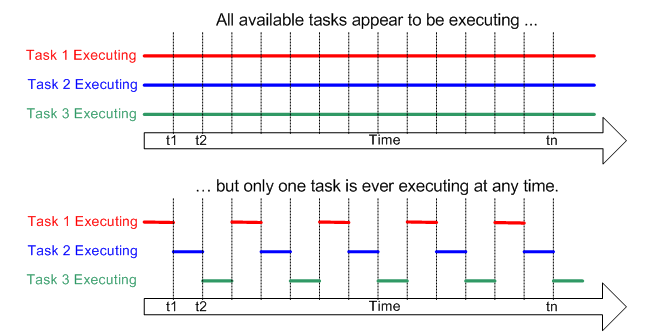
\includegraphics[scale=0.7]{RTOS/f1.PNG}
% \end{figure}